\documentclass[runningheads]{llncs}

\usepackage{proof}
\usepackage{stmaryrd}
\usepackage{amsmath}
\usepackage{amssymb}
\usepackage{listings}
\usepackage{varwidth}
\usepackage{tikz}
\usepackage{tikz-cd}
\usepackage{nameref}
\usepackage{caption}
\usepackage{subcaption}
\usepackage{empheq}
\usepackage[most]{tcolorbox}
% \usepackage{syntax}
% \usepackage{simplebnf}

\usetikzlibrary{backgrounds,fit,decorations.pathreplacing,calc}
\lstset{basicstyle=\ttfamily, mathescape=true, literate={~} {$\sim$}{1}}

\definecolor{lightgreen}{HTML}{90EE90}

% Based on https://tex.stackexchange.com/a/288326/186240
\newtcbox{\condition}[1][]{%
    nobeforeafter, math upper, tcbox raise base,
    enhanced, colframe=blue!30!black,
    colback=lightgreen, boxrule=1pt,
    #1}

\newcommand {\ite} {\textsf{if}}
\newcommand {\Ra} {\Rightarrow}
\newcommand {\deref} {\textsf{deref}}
\newcommand {\apply} {\textsf{apply}}
\newcommand {\ra} {\rightarrow}
\newcommand {\labinfer} [3] [] {\infer[{\textsc{#1}}]{#2}{#3}}
\newcommand {\Type} {\textsf{Type}}
\newcommand {\Nat} {\textsf{Nat}}
\newcommand {\Bool} {\textsf{Bool}}
\newcommand {\Vect} {\textsf{Vec}}
\newcommand {\ok} {\text{ type}}
\newcommand {\Env} {\textsf{Env}}
\newcommand {\State} {\textsf{State}}
\newcommand {\Value} {\textsf{Value}}
\newcommand {\Locus} {\textsf{Locus}}
\newcommand {\Loc} {\textsf{Location}}
\newcommand {\sem} [1] {\llbracket #1 \rrbracket}
\newcommand {\Esem} [1] {E\sem{#1}}
\newcommand {\Expr} {\textsf{Expr}}
\newcommand {\Cmd} {\textsf{Stmt}}
\newcommand {\CmdTy} {\texttt{Stmt}}
\newcommand {\ExprTy} {\texttt{ExprTy}}
\newcommand {\Apply} {\textsf{Apply}}
\newcommand {\fst} {\ensuremath{\textsf{proj}_1}}
\newcommand {\snd} {\ensuremath{\textsf{proj}_2}}
\newcommand {\Var} {\textsf{Var}}
\newcommand {\Index} {\textsf{Index}}
\newcommand {\Cast} {\textsf{Cast}}
\newcommand {\Rename} {\textsf{Rename}}
\newcommand {\Permute} {\textsf{Permute}}
\newcommand {\loceq} {\approx}
\newcommand {\sep} {\ast}
\newcommand {\pointsto} {\mapsto}

\newcommand{\ket}[1]{\ensuremath{\left|#1\right\rangle}}

\begin{document}

\title{QSym from the Ground Up}
\author{}
\institute{}
\maketitle

\section{Circuit Basics}

A quantum operator is drawn in the following way in a quantum circuit. We have the convention that information flows from left-to-right. In this
case, $q$ is the name of the input and $q'$ is the name of the output. $F$ is the name of the linear transformation.

\begin{figure}[h]
  \centering
\begin{minipage}{.5\textwidth}
  \centering
% Based on https://tex.stackexchange.com/a/44270/186240
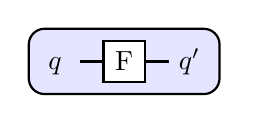
\begin{tikzpicture}[thick]
    % `operator' will only be used by Hadamard (H) gates here.
    % `phase' is used for controlled phase gates (dots).
    % `surround' is used for the background box.
    \tikzstyle{operator} = [draw,fill=white,minimum size=1.5em] 
    \tikzstyle{phase} = [draw,fill,shape=circle,minimum size=5pt,inner sep=0pt]
    \tikzstyle{surround} = [fill=blue!10,thick,draw=black,rounded corners=2mm]
    %
    \matrix[row sep=0.4cm, column sep=0.8cm] (circuit) {
      \node (q0) {$q\phantom{'}$}; &[-0.5cm] 
      \node[operator] (op) {F}; &[-0.5cm] 
      \node (q1) {$q'$}; &[-0.5cm] 
    \coordinate (end0); \\
    %
  };
  \begin{pgfonlayer}{background}
        % Draw background box.
    \node[surround] (background) [fit = (q0) (op) (q1) ] {};
        % Draw lines.
        \draw[thick] (q0) -- (op)   (op) -- (q1);
    \end{pgfonlayer}
\end{tikzpicture}
\end{minipage}
\end{figure}

\subsection{Serial composition}

Serial composition is given by composition of operators. In the matrix representation, this is matrix multiplication. $G \circ F$ is also often written $GF$.

\begin{figure}[h]
  \centering
\begin{minipage}{.5\textwidth}
  \centering
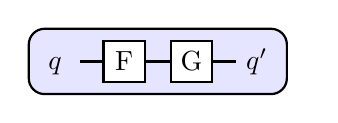
\begin{tikzpicture}[thick]
    % `operator' will only be used by Hadamard (H) gates here.
    % `phase' is used for controlled phase gates (dots).
    % `surround' is used for the background box.
    \tikzstyle{operator} = [draw,fill=white,minimum size=1.5em] 
    \tikzstyle{phase} = [draw,fill,shape=circle,minimum size=5pt,inner sep=0pt]
    \tikzstyle{surround} = [fill=blue!10,thick,draw=black,rounded corners=2mm]
    %
    \matrix[row sep=0.4cm, column sep=0.8cm] (circuit) {
      \node (q0) {$q\phantom{'}$}; &[-0.5cm] 
      \node[operator] (op0) {F}; &[-0.5cm] 
      \node[operator] (op1) {G}; &[-0.5cm] 
      \node (q1) {$q'$}; &[-0.5cm] 
    \coordinate (end0); \\
    %
  };
  \begin{pgfonlayer}{background}
        % Draw background box.
    \node[surround] (background) [fit = (q0) (op0) (op1) (q1) ] {};
        % Draw lines.
        \draw[thick] (q0) -- (op0)   (op0) -- (op1)   (op1) -- (q1);
    \end{pgfonlayer}
\end{tikzpicture}
\end{minipage}
  \caption{$G \circ F$}
\end{figure}

\subsection{Parallel composition}

Putting two components side-by-side in the circuit corresponds to the tensor product of the operators that the components represent. In
the matrix representation, the tensor product is given by the Kronecker product of the two matrices.

\begin{figure}[h]
  \centering
\begin{minipage}{.5\textwidth}
    \centering
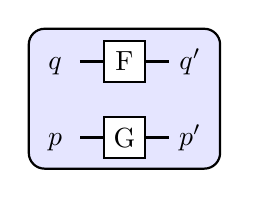
\begin{tikzpicture}[thick]
    % `operator' will only be used by Hadamard (H) gates here.
    % `phase' is used for controlled phase gates (dots).
    % `surround' is used for the background box.
    \tikzstyle{operator} = [draw,fill=white,minimum size=1.5em] 
    \tikzstyle{phase} = [draw,fill,shape=circle,minimum size=5pt,inner sep=0pt]
    \tikzstyle{surround} = [fill=blue!10,thick,draw=black,rounded corners=2mm]
    %
    \matrix[row sep=0.4cm, column sep=0.8cm] (circuit) {
      \node (q0) {$q\phantom{'}$}; &[-0.5cm] 
      \node[operator] (op0) {F}; &[-0.5cm] 
      \node (q1) {$q'$}; &[-0.5cm] 
    \coordinate (end0); \\

      \node (p0) {$p\phantom{'}$}; &[-0.5cm] 
      \node[operator] (op1) {G}; &[-0.5cm] 
      \node (p1) {$p'$}; &[-0.5cm] 
    \coordinate (end1); \\
    %
  };
  \begin{pgfonlayer}{background}
        % Draw background box.
    \node[surround] (background) [fit = (q0) (op0) (op1) (q1) ] {};
        % Draw lines.
        \draw[thick] (q0) -- (op0)   (op0) -- (q1)
                     (p0) -- (op1)   (op1) -- (p1);
    \end{pgfonlayer}
\end{tikzpicture}
\end{minipage}
  \caption{$F \otimes G$}
\end{figure}

\subsection{The interchange law}

The interchange law says it doesn't matter if we, given four components, we first put two pairs side-by-side and then
hook them up each other, or if we hook them up to each other first. This results in the exact same circuit diagram. We can
write it in two different ways symbolically, and we say that the following equation holds. This is the interchange law.

\[
  (S \otimes T) \circ (F \otimes G) = (S \circ F) \otimes (T \circ G)
\]

The circuit notation has the advantage that this equality always holds implicitly. We never need to actually use it, if we are
drawing circuits (unlike the symbolic notation).

\begin{figure}[h]
  \centering
\begin{minipage}{.5\textwidth}
    \centering
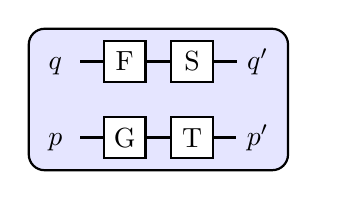
\begin{tikzpicture}[thick]
    % `operator' will only be used by Hadamard (H) gates here.
    % `phase' is used for controlled phase gates (dots).
    % `surround' is used for the background box.
    \tikzstyle{operator} = [draw,fill=white,minimum size=1.5em] 
    \tikzstyle{phase} = [draw,fill,shape=circle,minimum size=5pt,inner sep=0pt]
    \tikzstyle{surround} = [fill=blue!10,thick,draw=black,rounded corners=2mm]
    %
    \matrix[row sep=0.4cm, column sep=0.8cm] (circuit) {
      \node (q0) {$q\phantom{'}$}; &[-0.5cm] 
      \node[operator] (op0) {F}; &[-0.5cm] 
      \node[operator] (op1) {S}; &[-0.5cm] 
      \node (q1) {$q'$}; &[-0.5cm] 
    \coordinate (end0); \\

      \node (p0) {$p\phantom{'}$}; &[-0.5cm] 
      \node[operator] (op2) {G}; &[-0.5cm] 
      \node[operator] (op3) {T}; &[-0.5cm] 
      \node (p1) {$p'$}; &[-0.5cm] 
    \coordinate (end1); \\
    %
  };
  \begin{pgfonlayer}{background}
        % Draw background box.
    \node[surround] (background) [fit = (q0) (op0) (op1) (q1)
                                        (p0) (op2) (op3) (p1) ] {};
        % Draw lines.
        \draw[thick] (q0) -- (op0)  (op0) -- (op1)  (op1) -- (q1)
                     (p0) -- (op2)  (op2) -- (op3)  (op3) -- (p1);
    \end{pgfonlayer}
\end{tikzpicture}
\end{minipage}
  \caption{This is both $(S \otimes T) \circ (F \otimes G)$ and also $(S \circ F) \otimes (T \circ G)$}
\end{figure}

\section{Quantum states}

\subsection{Entanglement: A fictional simplification}

Imagine that we are using classical probability, and that the circuit describes a probabilistic machine.

We can talk about how the probabilities are transformed by the operators in the circuit. Now imagine that we have a
deterministic operator which takes in one bit and produces two outputs by duplicating the input bit. This does not correspond to an operator in a quantum circuit and is just for illustration purposes.
\\

\begin{minipage}{.5\textwidth}
    \centering
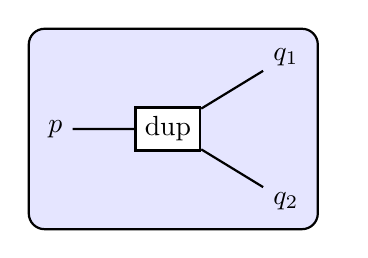
\begin{tikzpicture}[thick]
    % `operator' will only be used by Hadamard (H) gates here.
    % `phase' is used for controlled phase gates (dots).
    % `surround' is used for the background box.
    \tikzstyle{operator} = [draw,fill=white,minimum size=1.5em] 
    \tikzstyle{phase} = [draw,fill,shape=circle,minimum size=5pt,inner sep=0pt]
    \tikzstyle{surround} = [fill=blue!10,thick,draw=black,rounded corners=2mm]
    %
    \matrix[row sep=0.4cm, column sep=0.8cm] (circuit) {
      &&\node (q0) {$q_1$}; &[-0.5cm] 
    \coordinate (end0); \\

      \node (p0) {$p$}; &[-0.5cm] 
      \node[operator] (op0) {dup}; &[-0.5cm] 
    \coordinate(end1); \\

      &&\node (q1) {$q_2$}; &[-0.5cm] 
    \coordinate (end2); \\
    %
  };
  \begin{pgfonlayer}{background}
        % Draw background box.
    \node[surround] (background) [fit = (q0) (op0) (p0) (q1) ] {};
        % Draw lines.
        \draw[thick] (p0) -- (op0)   (op0) -- (q0)   (op0) -- (q1);
    \end{pgfonlayer}
\end{tikzpicture}
\end{minipage}
\\

Say we provide an input that has an even chance of being either a 0 or a 1. What is the probability of a 1 appearing at each of the two outputs?
We run into a problem trying to talk about the probabilities in isolation like this. If we say that output $q_1$ has a 1 with probability
$a$ and output $q_2$ has a 1 with probability $b$, we would expect that the output $10$ would have probability $q_1 \cdot (1 - q_2)$. When
we provide an input of $1$ with probability $1/2$, we find the probability of $10$ is $0.5 \cdot (1 - 0.5) = 0.25$. But an
output of $10$ isn't even possible! The operator only duplicates the input. What went wrong?

The two outputs are \textit{correlated} with each other. Instead of trying to look at the probabilities of the two outputs in isolation, we can
instead say that the output $00$ as a probability of $1/2$ and the output $11$ has a probability of $1/2$ (recall that we are providing it an input of $1$ with probability $1/2$).

This is analogous to how entanglement works in the case of a quantum circuit.


\end{document}
